\documentclass[a4paper,10pt]{article} \usepackage{anysize}
\marginsize{2cm}{2cm}{1cm}{1cm}
%\textwidth 6.0in \textheight = 664pt
\usepackage{xltxtra}
\usepackage{xunicode} \usepackage{graphicx}
\usepackage{color} \usepackage{xgreek} \usepackage{fancyvrb}
\usepackage{minted}
\usepackage{listings}
\usepackage{enumitem} \usepackage{framed} \usepackage{relsize}
\usepackage{float} \setmainfont[Mapping=TeX-text]{CMU Serif}
\begin{document}

\begin{titlepage}
\begin{center}
\begin{figure}[h] 
     
\includegraphics[width=0.2\textwidth]{title/ntua_logo}
\end{figure}
\vspace{1cm}
\begin{LARGE}\textbf{ΕΘΝΙΚΟ ΜΕΤΣΟΒΙΟ ΠΟΛΥΤΕΧΝΕΙΟ\\[1.5cm]}\end{LARGE}
\begin{Large}
ΣΧΟΛΗ ΗΜ\&ΜΥ\\
Εργαστήριο Μικροϋπολογιστών\\[2cm]
6\textsuperscript{η} Εργαστηριακή Άσκηση\\
Ακ. έτος 2011-2012\\
\end{Large}
\vfill
\begin{flushright}
\Large \textit{Ομάδα C07:}\\[1cm]
\begin{tabular}{l r}
{Ελένη \textsc{Ευαγγελάτου}}&
{Α.Μ.: 03108050}\\
{Γρηγόρης \textsc{Λύρας}}&
{Α.Μ.: 03109687}\\
{Βασιλεία \textsc{Φραγκιαδάκη}}&
{Α.Μ.: 03108026}\\
\end{tabular}
\end{flushright}

\large\today\\
\end{center}
\end{titlepage}




\section*{} 
\subsection*{Άσκηση 3(i)}
Σε αυτήν την άσκηση υλοποιούμε την εξομοίωση του εξής ολοκληρωμένου
κυκλώματος:
\begin{figure}[h]
\centering
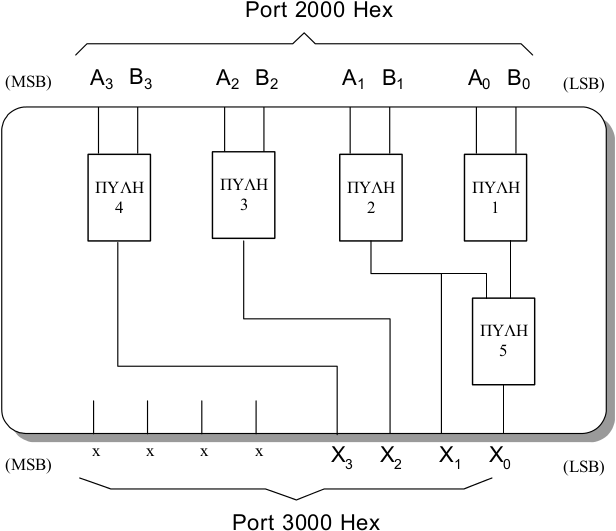
\includegraphics[width=0.7\textwidth]{files/ask_3_i_IC.png}
\caption{Το IC του θέματος}
\end{figure}
Για την διαδικασία που ακολουθήσαμε αποθηκεύσαμε το αποτέλεσμά μας στον C,
έχοντας ως βοηθητικό buffer τον B και κάνοντας πράξεις στον Α. Αρχικά
παίρνουμε ένα ένα ψηφίο από την είσοδο μας απομονώνοντάς το με RAL και
βλέπουμε το κρατούμενο. Υλοποιούμε σε πρώτο βήμα τις 4 πύλες XOR. Για να
υλοποιήσουμε την κάθε πύλη ουσιαστικά κοιτάμε αν έχουμε 0 με 1 (ή 1 με 0) στα
συγκρινόμενα ψηφία, οπότε και η XOR δίνει αποτέλεσμα TRUE (δηλαδή 1) . Αυτήν
την πράξη επαναλαμβάνουμε και για τα 8 bits της εισόδου (φυσικά σε ζεύγη, όπως
δίνονται στο σχήμα). Το αποτέλεσμα αποθηκεύεται στον C. Σε δεύτερο στάδιο
αποθηκεύουμε τα δύο τελευταία least significant bits και τα βάζουμε ως
τελεστέους σε μία OR. Αφού προηγουμένως "αδειάσουμε" το lsb του C ,
αποθηκεύουμε εκεί το αποτέλεσμα της OR. Το τελικό αποτέλεσμα περνιέται εκ νέου
στον C και τα περιεχόμενα του οποίου εμφανίζουμε στα LEDS.

Ο κώδικάς μας είναι ο εξής:
\inputminted[linenos,obeytabs,frame=leftline,fontsize=\footnotesize]{oldasm}{files/askhsh_3_i.8085}
\subsection*{Άσκηση 4(ii)}
Σε αυτή την άσκηση ζητείται να απεικονίσουμε στα δύο αριστερότερα displays την
τιμή του κωδικού του πλήκτρου που πατήθηκε σύμφωνα με τον πίνακα 1 (στη σελ.
82 του βιβλίου). Γι' αυτό το σκοπό πρώτα σβήνουμε τελείως όλα τα displays,
φορτώνοντας στις θέσεις μνήμης 0ΒΒ0Η-0ΒΒ5Η τη δεκαεξαδική τιμή 10Η (αφού
έχουμε άρει την προστασία μνήμης) και καλώντας τη ρουτίνα STDM που μεταφέρει
τα δεδομένα από εκεί που τα έχουμε αποθηκεύσει, στις θέσεις μνήμης που θα τα
βρει η DCD. Έπειτα η KIND φορτώνει στον Α τον κωδικό του πλήκτρου που
πατήθηκε. Για να τον απεικονίσουμε, απομονώνουμε τα τέσσερα lsb και τα
φορτώνουμε στη θέση μνήμης που αντιστοιχεί στο 5ο ψηφίο και τα msb που
φορτώνουμε στη θέση μνήμης που αντιστοιχεί στο 6ο ψηφίο. Έπειτα, με την κλήση
διαδοχικά των STDM και DCD απεικονίζεται στα diplays ο ζητούμενος κωδικός. Να
σημειώσουμε ότι η KIND στο σώμα της, όπου υπάρχει αναμονή, καλεί συνεχώς τη
DCD και έτσι "φρεσκάρεται" η οθόνη.

Ο κώδικάς μας φαίνεται παρακάτω:
\inputminted[linenos,obeytabs,frame=leftline,fontsize=\footnotesize]{oldasm}{files/askhsh_4_ii.8085}
\subsection*{Άσκηση 4(iv)}
Η λογική μας σε αυτήν την άσκηση είναι ότι από τον δοθέντα αριθμό μετρήσαμε
τις εκατοντάδες (που μπορεί να είναι μία ή μηδέν, διότι το πολύ μέχρι 127 θα
μετρήσουμε κατά την εκφώνηση της άσκησης), τις δεκάδες και τις μονάδες και το
πρόσημο του αριθμού. Οι εκατοντάδες, δεκάδες και μονάδες του αριθμού
αποθηκεύονται στους καταχωρητές  D, B, C αντίστοιχα, ενώ το πρόσημο στον E. Οι
αριθμοί που δίνονται είναι από -128 έως 127.\\

\begin{figure}[h]
\centering
\begin{tabular}{r r r r r r r r r r}
MSB &&&&&&&\\
0 & 1 & 1 & 1 & 1 & 1 & 1 & 1 & = & 127\\
0 & 1 & 1 & 1 & 1 & 1 & 1 & 0 & = & 126\\
0 & 0 & 0 & 0 & 0 & 0 & 1 & 0 & = & 2\\
0 & 0 & 0 & 0 & 0 & 0 & 0 & 1 & = & 1\\
0 & 0 & 0 & 0 & 0 & 0 & 0 & 0 & = & 0\\
1 & 1 & 1 & 1 & 1 & 1 & 1 & 1 & = & -1\\
1 & 1 & 1 & 1 & 1 & 1 & 1 & 0 & = & -2\\
1 & 0 & 0 & 0 & 0 & 0 & 0 & 1 & = & -127\\
1 & 0 & 0 & 0 & 0 & 0 & 0 & 0 & = & -128\\
%& 1 & 1 & 1 &
\end{tabular}
\caption{Πίνακας τιμών}
\end{figure}

Για να γίνει αυτή η διαδικασία, βλέπουμε αν ο αριθμός μας είναι θετικός ή
αρνητικός από το msb του. Εφόσον είναι θετικός αποθηκεύουμε στον Ε τον κωδικό
της DCD ,10, ο οποίος αντιστοιχεί σε (κενό). Αν είναι αρνητικός τότε
αποθηκεύουμε τον κωδικό 1C στον E, γιατί αυτός αντιστοιχεί σε μείον (-) στην
DCD . Επίσης για να χειριστούμε τον  υπόλοιπο αρνητικό αριθμό (ο οποίος είναι
σε συμπλήρωμα ως προς 2), παίρνουμε το συμπλήρωμα ως προς 1 και προσθέτουμε 1.
Αυτό το κάνουμε διότι το συμπλήρωμα ως προς 2 του συμπληρώματος ως προς 2 μας
δίνει τον αρχικό (θετικό) αριθμό. Στην συνέχεια για να μετρήσουμε τις
εκατοντάδες, δεκάδες και μονάδες, κοιτάμε αν ο αριθμός μας είναι μεγαλύτερος
του 100. Αν ναι μετράμε μία εκατοντάδα και αφαιρούμε από τον αριθμό 100.
Έπειτα (ή και αν ο αριθμός είναι <100) μετράμε πόσες δεκάδες έχουμε. Αφαιρούμε
10   έως ότου να έχουμε αρνητικό αριθμό και μετράμε πόσες φορές αφαιρέσαμε 10.
μΕτά προσθέτουμε 10 για την διόρθωση του υπολοίπου. Το διορθωμένο υπόλοιπο
είναι οι μονάδες. Αποθηκεύουμε τους καταχωρητές σε 6 συνεχόμενες θέσεις μνήμης
(4 οι καταχωρητές + 2 με κωδικούς 10 για κενό, ώστε να μην εμφανίζουν τίποτε).
Πλέον καλούμε την  STDM , αφού της “γνωστοποιούμε” που είναι αυτές οι 6 θέσεις
μνήμης και καλούμε και την DCD για την εμφάνιση στα 7segments και έχουμε τον
αριθμό σε δεκαδική μορφή μαζί με το πρόσημο στα 7 segments.


\inputminted[linenos,obeytabs,frame=leftline,fontsize=\footnotesize]{oldasm}{files/askhsh_4_iv.8085}
\end{document}
